\section*{目录}

\subsection{1 分布式共识回顾}

\textbf{什么是分布式共识：}每个进程都提出一个值。所有进程必须就其中一个提议值达成一致。

例子：
\begin{itemize}
\item 将军们必须就进攻时间达成一致
\item 分布式数据存储中跨多个服务器复制的对象，所有服务器必须就对象的当前版本达成一致
\item 在复制服务器上进行事务处理必须就对象更新的顺序达成一致
\end{itemize}

\subsection{FLP 定理}

\textbf{FLP 不可能性：}在异步-崩溃-停机系统模型中，不存在保证能终止的共识算法。

原文：
\begin{quote}
``The consensus problem involves an asynchronous system of processes, some of which may be unreliable. ... In this paper, it is shown that every protocol for this problem has the possibility of non-termination, even with only one possibly faulty process.''
\end{quote}
在一个完全异步的消息传递分布式系统中，其中即使只有一个发送崩溃故障，不可能存在达成共识的确定性算法。Fischer, Lynch 和 Paterson 在 1985 年著名的 FLP 不可能性结果中给予了证明。

\subsection{共识算法的设计目标}

一个完美的共识算法必须满足以下性质：
\begin{itemize}
\item \textbf{安全性 (Safety):} 任何时候都不会达成错误的共识（例如，两个不同的值被决议为‘共识’）。
  内涵包括：
  \begin{itemize}
  \item 一致性：所有诚实进程决定的值必须相同。 $\forall i, j \in \text{Correct}: d_i = d_j$。
  \item 确定性进程可能会：最终决定的值 $v$ 必须是由某个进程提出的初始值。 $v \in \{v_1, v_2, \dots, v_n\}$。
  \end{itemize}
\item \textbf{活性 (Liveness):} 不能陷入永久停滞。
  内涵为：
  \begin{itemize}
  \item 终止性 (Termination): 每一个诚实的进程最终都会在有限时间内完成决策。
  \end{itemize}
\end{itemize}

\subsection{FLP 定理的视角}

在完全异步系统中，没有任何确定性算法能同时严格满足上述两方面性质。
现有分布式共识算法如 Paxos 和 Raft 选择了在极端情况下牺牲 Liveness（活性）以绝对保证 Safety（安全性）。
为什么？如果强行要求活性，节点可能会在信息不足的情况下做出“猜测”，从而破坏安全性。

\section{2 Paxos}

\subsection{Paxos 共识算法}

异步系统中共识的 Paxos 算法。
\begin{itemize}
\item 最流行的共识算法。
\item Zookeeper, Google Chubby, 以及许多系统使用它。
\item 基本思想：一旦多数人同意一项提案，就达成共识。达成的共识最终为所有成员悉知。
\end{itemize}

猜猜是谁发明的？ Leslie Lamport! 原始论文: ``The Part-time Parliament''，使用了希腊 Paxos 岛上“兼职议会”的类比。该论文发表后难以理解。 1 年后发表了 ``Paxos made simple''。
参考：
\begin{itemize}
\item Leslie Lamport. The part-time parliament. ACM Transactions on Computer Systems (TOCS), Volume 16, Issue 2 Pages 133 -169
\item Leslie Lamport. (2001). Paxos Made Simple. ACM SIGACT News (Distributed Computing Column) 32, 4 (Whole Number 121, December 2001) pp. 51-58
\end{itemize}

\subsubsection{Paxos 共识算法: 角色划分}

角色: Paxos 将系统成员划分为三个角色: 提议者 (Proposer), 接受者 (Acceptor)，决策学习者 (Learner)

阶段: Paxos 算法决议过程包含三个阶段:
\begin{itemize}
\item 第一阶段: Prepare phase 准备阶段
\item 第二阶段: Accept phase 接受阶段
\item 第三阶段: Learn phase 学习阶段
\end{itemize}

提案: 包括提案编号 (Proposal ID) 和提议值 (Value); 提案指令，记为: $[n, v]$

\subsubsection{Paxos 共识算法: 提案编号}

允许接受者回应多个提案。
\begin{itemize}
\item 回应与接受：接受者 (Acceptor) 确实可以先后回复多个提案，但一旦某个提案被多数派 (Quorum) 接受，则达成共识，后续提案必须沿用该值。
\item 为不同进程配置不相交的可能提案编号集合。
\item 提案编号全序：高编号提案具有更高的优先级，可以令尚未达成的低编号提案失效。
\item 高编号会使接受者承诺不再批准任何低编号的提案（抢占）。
\item 如果提议者在准备阶段发现了已存在的值，它必须放弃自己的值，转而提议这个发现的高编号值。（确保 Safety）
\end{itemize}

\subsubsection{Paxos 共识算法: 三类角色}

三类角色（一个进程可以有多个角色）:
\begin{itemize}
\item 提议者 (Proposers): 向接受者提议值。
  \begin{itemize}
  \item 算法发起者，驱动协商进程
  \item 接受应用层请求，将请求封装为一个提案 (Proposal)
  \item 发送提案，将提案发送给所有接受者
  \item 根据响应，决定后续工作
  \end{itemize}
\item 接受者 (Acceptors): 接受提议的值 (在某些条件下)。
  \begin{itemize}
  \item 回应提议者的提案，根据规则进行投票表决。
  \item 处理: Prepare Request (准备请求) 和 Accept Request (接受请求)
  \item 选择: 多数 Acceptors 接受某 Accept Request，达成共识
  \end{itemize}
\item 学习者 (Learners): 学习已被多数接受者接受的值。
  \begin{itemize}
  \item 不参加提案发送与决策
  \item 采纳提议者/接受者最新达成一致的提案 (Value)
  \item 可根据实际需求，实现其它功能
  \end{itemize}
\end{itemize}

这里的多数意味着绝对多数（也包括崩溃的进程），假设崩溃的进程可以再次恢复。

\subsubsection{Paxos 算法: 尝试单阶段方案}

提议者将其提议的值组播到足够大的集合（大于多数派）的接受者。
\begin{itemize}
\item 接受者接受它收到的第一个提议值。如果多数接受者接受了相同的值 $v$，那么 $v$ 就是决定的值。
\item 这里可能会出什么问题？
  \begin{enumerate}
  \item 无法应对“提案冲突” (Race Condition)
  \item 无法处理“旧提案的滞后覆盖” (Stale Updates)，网络延迟是无法避免的
  \item 破坏安全性 (Safety Violation)
  \end{enumerate}
\end{itemize}

\subsubsection{Paxos: 算法 (Prepare 阶段)}

提议者: 选择一个提案编号 $M$，将 prepare request 发送给多数派接受者。$M$ 是全局唯一且单调递增的。

接受者: 收到 Prepare 请求后，根据规则响应:
\begin{itemize}
\item 如果 $M$ 大于此接受者已经回复的准备请求中的最大提案编号，则:
  \begin{itemize}
  \item 承诺在当前准备请求的响应中，不会回复并承诺任何编号较低的其他提案。
  \item 同时让提议者知道之前的共识状态: 反馈已接受的 Accept 请求中最大编号的提案指令；如果没有接受任何 Accept 请求，则反馈 Nil。
  \end{itemize}
\item 如果 $M$ 小于等于接受者已经回复的准备请求中最大提案编号，则拒绝本次 Prepare 请求，不回复提议者。
\end{itemize}

注意: 响应 Nil 和不响应并不相同。

\subsubsection{Paxos: 算法 (Accept 阶段)}

提议者: 如果提议者从多数接受者收到其准备请求 $M$ 的响应，则:
\begin{itemize}
\item 向每个这些接受者发送带有提议值的接受请求 (accept request)，请求包含提案编号和提案指令，记为 $[m, v]$。
\item 如果提议者没有听到多数接受者的响应怎么办？等待一段时间，然后发出带有更高编号的新请求。
\end{itemize}

接受者: 收到提案 $[m, v]$ 的接受请求后，根据以下约定对 Proposer 反馈:
\begin{itemize}
\item 如果接受者没有回复编号大于 $m$ 的 Prepare 请求，则接受提案 $[m, v]$，并返回已接受的最大编号。
\item 如果接受者已经回复编号为 $Y$ 的 Prepare 请求，且 $M < N$，则拒绝该 Accept 请求，回复 No。
\item 在下一轮协商中，提议者可以基于上述响应中的提案编号进行递增，而不用尝试逐个递增。
\item 如果多数接受者接受了该 Accept 请求，则记作提案 $[m, v]$ 已被选择或者达成共识。如果没有多数的接受者批准该 Accept 请求，则退回 Prepare 阶段重新协商。
\end{itemize}

\textbf{Paxos: 算法 (Accept 阶段) 中的值确定:}
\begin{itemize}
\item 如果在 Prepare 请求响应中，部分接受者反馈了提案指令，则 $v$ 为 Prepare 请求反馈中最大提案编号对应的提案指令，即使这不是提议者的初衷（保证“一旦选定，不可更改”）。
\item 否则，$v$ 可以由提议者任意指定。
\end{itemize}

\subsubsection{Paxos: 算法 (Learn 阶段)}

Learn 阶段不属于 Paxos 的协商阶段，将达成共识提案交给学习者，由其做相应操作。

学习者如何知晓已达成的共识提案?
\begin{enumerate}
\item 由 Proposer 同步: (最简方案) 只有提议者知道提案是否已达成共识和最终共识提案，如果已达成共识，Proposer 则立即将该提案发送给学习者。
\item 接受者转发 Accept 请求给学习者: 当接受者批准一个 Accept 请求时，将其转发给学习者，由其判断是否有多数接受者批准同一请求，以此决定如何操作（状态转移等）。
\item 接受者之间交换已批准的 Accept 请求: 当接受者批准一个 Accept 请求时，将其广播给其他接受者，则所有接受者都能判断提案是否已达成共识，并将共识提案发给学习者。明显又增加了一轮消息交互，但是，每个接受者都有已达成共识的标志，使得读请求不必再执行一轮协商。
\end{enumerate}

\subsection{Paxos 算法 FAQ}

如果我们有多个提议者怎么办?
\begin{itemize}
\item 两个提议者可能通过不断发送带有更高编号的新提案来抢占彼此的请求（活锁）。
\item 这里给大家演示一下活锁。
\item 安全性仍然得到保证!
\end{itemize}

如果多数接受者在值决定之前失败怎么办?
\begin{itemize}
\item 算法不终止。
\item 安全性仍然得到保证!
\end{itemize}

如果进程失败并再次恢复怎么办?
\begin{itemize}
\item 如果它是接受者，它必须记住它已接受的最高编号提案。接受者将接受的提案记录在磁盘上。
\item 只要此状态可以在故障和恢复后检索，算法就能正常工作，安全性仍然得到保证。
\end{itemize}

\subsection{日志共识}

\begin{itemize}
\item Paxos 算法（到目前为止讨论的）用于决定单个值。
\item 许多实际系统需要决定一系列值（日志）。
\item 复制日志 => 复制状态机。所有服务器以相同顺序执行相同命令。共识模块确保正确的日志复制。
\item 日志共识: Multi-Paxos: 对每个日志条目重复运行 Paxos。
  \begin{itemize}
  \item 很快变得非常复杂。
  \item 性能优化进一步增加了复杂性。
  \end{itemize}
\end{itemize}

\subsection{Paxos 的效率问题}

使用 Basic Paxos 效率较低:
\begin{itemize}
\item 多 Proposer 竞争
\item 多次 RPC (Prepare + Accept)
\end{itemize}
解决方案:
\begin{enumerate}
\item 选举 leader
\item 消除大多数 Prepare RPC
\end{enumerate}
优化方式:
\begin{itemize}
\item 对整个日志执行一次 Prepare（而不是每个条目）
\item 之后只运行 Accept
\end{itemize}

\subsection{Multi-Paxos 运行流程}

\subsubsection{阶段 A: Leader 选举 (Prepare)}
\begin{itemize}
\item 选择一个 Leader，并发送 Prepare(?, $m$)。
\item 一旦获得多数派承诺，该 Leader 拥有后续所有实例的写入权。
\end{itemize}

\subsubsection{阶段 B: 稳态运行 (Accept)}
\begin{itemize}
\item Leader 直接发送 Accept(I, $v$)
\item 响应耗时从 2-RTT 降低到 1-RTT。
\end{itemize}
注: 稳态下只需蓝色箭头的 Accept 阶段。

\begin{figure}[htbp]
\centering
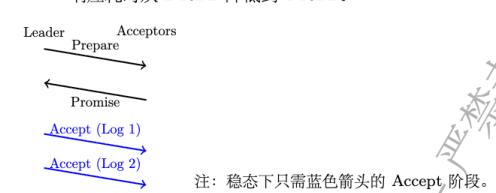
\includegraphics[width=0.8\textwidth]{figures/ch8/ch8_multipaxos_accept.png}
\caption{Multi-Paxos 稳态 Accept 阶段：Leader 向 Acceptors 复制日志}
\end{figure}

\subsection{总结}

\begin{itemize}
\item Basic Paxos: Prepare - Accept
\item Multi-Paxos: 包含 leader 选举、一次 Prepare、多次 Accept
\end{itemize}

\subsection{客户端协议、配置变更}

\subsection{对 Paxos 的批评}

\begin{quote}
``The dirty little secret of the NSDI community is that at most five people really truly understand every part of Paxos ;-).'' \hfill --- Anonymous NSDI Reviewer.
\end{quote}
\begin{quote}
``There are significant gaps between the description of the Paxos algorithm and the needs of a real-world system: ... the final system will be based on an unproven protocol.'' \hfill --- Chubby 作者
\end{quote}

\subsection{小结}

\begin{itemize}
\item 共识是分布式系统中的一个基本问题。
\item 可以在同步系统中解决共识。
  \begin{itemize}
  \item 基于时间同步轮次的算法。
  \item 需要至少 $(f+1)$ 轮来处理最多 $f$ 个故障。
  \end{itemize}
\item 不可能在异步系统中解决共识。
  \begin{itemize}
  \item 无法区分超时和非常非常慢的进程。
  \end{itemize}
\item Paxos 算法:
  \begin{itemize}
  \item 保证安全性但不保证活性。
  \item 希望在足够好的条件下终止。
  \end{itemize}
\end{itemize}

汇报完毕，欢迎同学们批评指教！
本次课涉及课程教材第?章，有大量补充内容。 % 需要指定章节
